\section{Enquadramento Teórico}

\subsection{Basic Myers List}

A Myers List original, proposta por Eugene W. Myers (1983) \cite{myers1983}, introduz um apontador \texttt{jump} adicional em cada célula de uma \textit{cons list}, 
permitindo \textit{lookup} em $3 \log( n ) - 5$ apontadores no pior caso. A sua construção iterativa preserva o suporte a \textit{cons} em tempo $\mathcal{O}(1)$, 
mas o seu desempenho assintótico fica aquém do limite teórico de informação.

\begin{figure}[H]
    \centering
    
    \subfloat[Formato de lista]{
        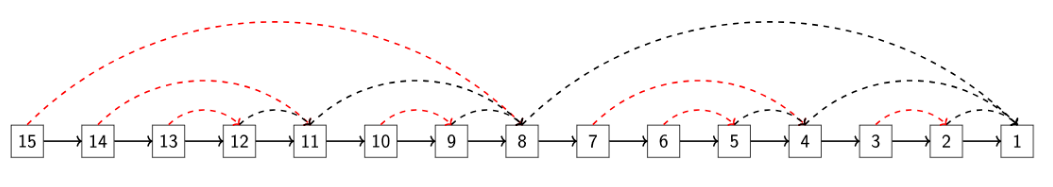
\includegraphics[width=0.48\linewidth]{Imagens/Basic-Lista}
    }
    \hfill
    \subfloat[Formato de árvore]{
        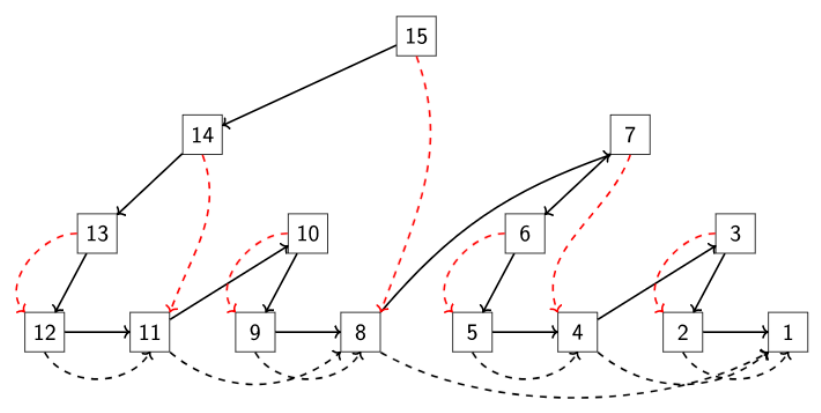
\includegraphics[width=0.4\linewidth]{Imagens/Basic-Arvore.png}
    }
    \caption{Representação da Basic Myers List}
    \label{fig:Basic}
\end{figure}

Assumindo as seguintes células, a associação do apontador \texttt{jump} para uma célula nova \(c\) funciona da seguinte forma:

\begin{figure}[H]
    \centering
    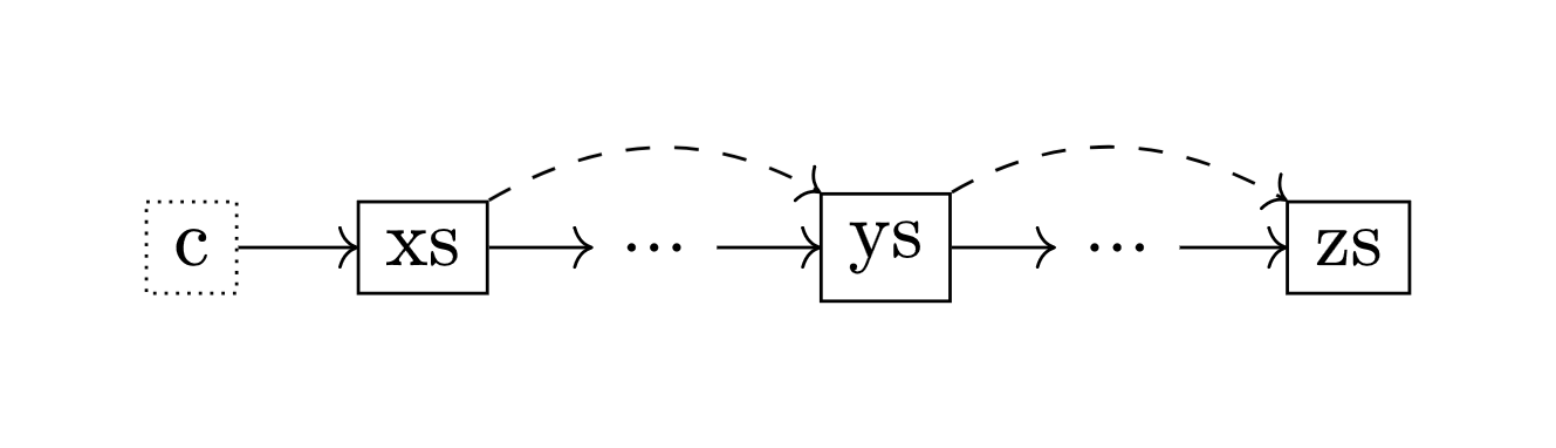
\includegraphics[width=0.5\linewidth]{Imagens/Basic-Cons}
    \caption{Exemplo de Basic Myers List, como células nomeadas}
    \label{fig:basic-cons}
\end{figure}

% Expressão matemática do jump
\begin{figure}[H]
    \centering
    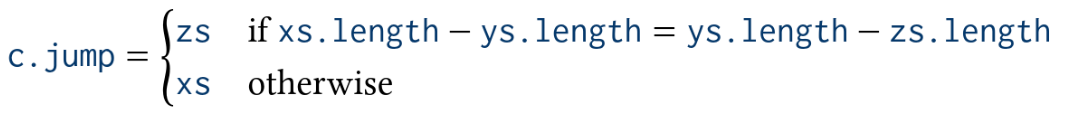
\includegraphics[width=0.5\linewidth]{Imagens/Basic-Jump} 
    \caption{\texttt{jump}}
    \label{fig:basic-jump}
\end{figure}

\textit{Lookup} na Basic Myers List é bastante simples, assume-se que \texttt{len} é um valor válido:

% Expressão matemática do lookup
\begin{figure}[H]
    \centering
    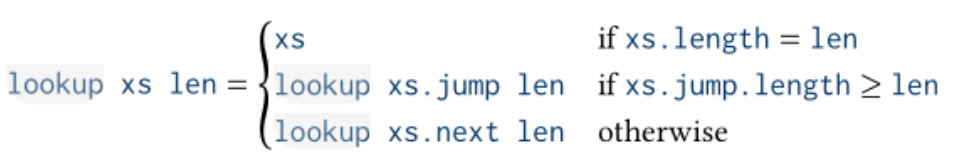
\includegraphics[width=0.5\linewidth]{Imagens/Basic-Lookup} 
    \caption{\textit{Lookup}}
    \label{fig:basic-lookup}
\end{figure}

\subsection{Improved Myers List}

A Improved Myers List, proposta por Peters, Foo e Adams (2025) \cite{peters2025}, introduz uma modificação simples, mas eficaz à maneira como a Basic Myers List é construída.
O apontador \texttt{jump} da primeira célula de cada região passa a apontar para a primeira célula da segunda sub-região, em vez da última 
célula. Assim, o resultado é uma melhoria do pior caso de \textit{lookup} de $3 \log(n) - 5$ para $2 \log(n + 1) - 3$ travessias, igualando ao desempenho da 
Okasaki List, estrutura de dados puramente funcional proposta por Chris Okasaki \cite{okasaki1995}, mas ainda com a vantagem de que permite o \textit{lookup} a partir de qualquer posição.

\begin{figure}[H]
    \centering
    
    \subfloat[Formato de lista]{
        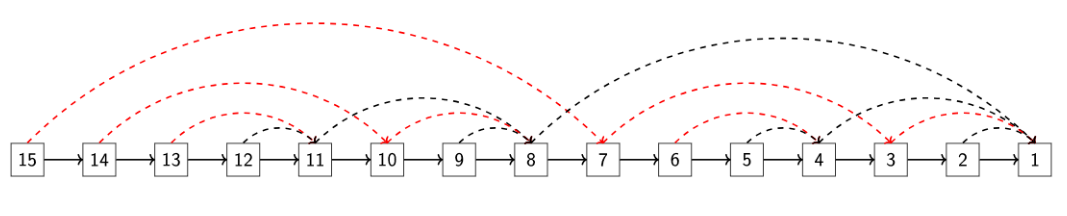
\includegraphics[width=0.48\linewidth]{Imagens/Improved-Lista}
    }
    \hfill
    \subfloat[Formato de árvore]{
        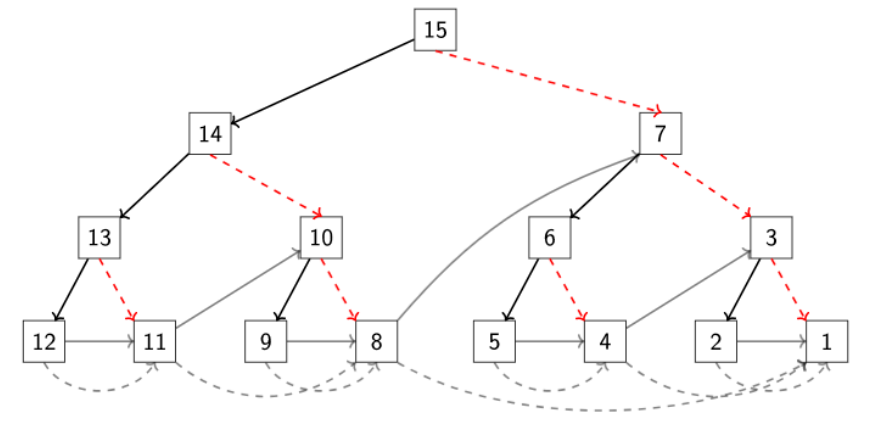
\includegraphics[width=0.4\linewidth]{Imagens/Improved-Arvore}
    }
    \caption{Representação da Improved Myers List}
    \label{fig:Improved}
\end{figure}


\subsubsection{Construção e conceito de região}

Uma região é definida pelo seu grau $k$:
\begin{itemize}
    \item Uma região de grau $k = 0$  consiste numa única célula.
    \item Uma região de grau $k > 0$ é composta por duas sub-regiões de grau $k - 1$ (no artigo, estas regiões são denominadas $Q_{k-1}$ e $R_{k-1}$) e uma célula adicional no início.
\end{itemize}

Na Basic Myers List, o apontador \texttt{jump} da célula inicial de uma região aponta para a última célula dessa mesma região. Adicionalmente, as duas 
sub-regiões partilham células, o que torna a estrutura menos eficiente.
A Improved Myers List resolve este problema alterando a regra de construção: as sub-regiões $Q_{k-1}$ e $R_{k-1}$ deixam de partilhar células, e o apontador 
\texttt{jump} da célula inicial passa a apontar diretamente para a primeira célula de $R_{k-1}$. Se visualizarmos a lista como uma árvore, as sub-regiões  $Q_{k-1}$ e 
$R_{k-1}$ formam, respetivamente, as sub-árvores esquerda e direita. Assim, o acesso à raiz da sub-árvore direita passa a custar apenas a travessia de 
um único apontador (\texttt{jump}), eliminando a ineficiência da variante clássica.

\begin{figure}[H]
    \centering
    \begin{tabular}{ccc}
        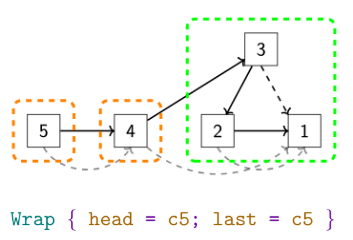
\includegraphics[width=0.3\linewidth]{Imagens/Regiao1} & 
        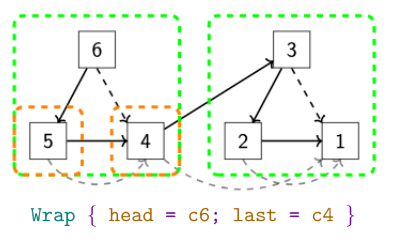
\includegraphics[width=0.3\linewidth]{Imagens/Regiao2} & 
        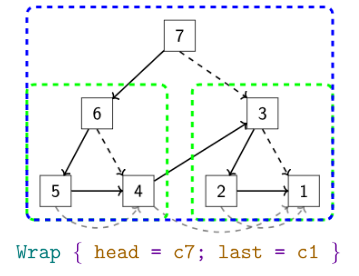
\includegraphics[width=0.3\linewidth]{Imagens/Regiao3}
    \end{tabular}
    \caption{Evolução do \texttt{wrap} durante o \textit{cons} na Improved Myers List}
    \label{tab:regioes}
\end{figure}

\subsubsection{\textit{Lookup}}

O algoritmo de \textit{lookup} na Improved Myers List é idêntico ao da Basic Myers List, percorre \texttt{jump} se \texttt{xs.jump.length} $\ge$ \texttt{len}, 
caso contrário, percorre \texttt{next}. 

\subsection{Advanced Myers List}

A Advanced Myers List, introduzida por Peters \cite{peters2025}, parte da Improved Myers List e introduz apontadores 
adicionais (\texttt{uncle}, \texttt{inc}, \texttt{greater}), permitindo assim um \textit{lookup} que pode ser realizado em tempo aproximadamente logarítmico 
$( 1 + \frac{1}{\sigma}) \log(n) + 9 + \sigma$ à custa de maior complexidade estrutural e de construção.


\begin{figure}[H]
    \centering
    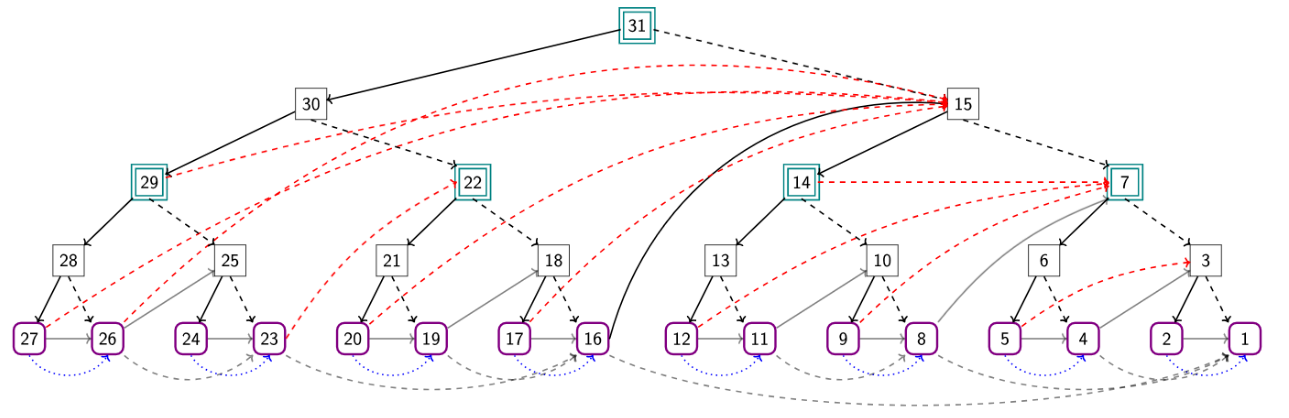
\includegraphics[width=0.8\linewidth]{Imagens/Advanced-Arvore} 
    \caption{Advanced Myers List}
    \label{fig:advanced}
\end{figure}

\subsubsection{Tipos de Nós}

A Advanced Myers List organiza as células em o que é chamado de nós lógicos, estes consistem em uma célula sozinha ou 
a junção de duas ou três células.
Existem três tipos de nós:
\begin{itemize}
    \item Nós normais -- são constituídos por apenas uma única célula (\textit{top}), contendo apontadores \texttt{next} e \texttt{jump} a apontar diretamente para os filhos esquerdo e direito.
    \item Nós \textit{skip} -- são constituídos por duas células, denominadas \textit{top} e \textit{bottom}. O apontador \texttt{next} da célula \textit{top} liga diretamente à célula bottom e o apontador \texttt{jump} aponta para o \texttt{uncle}. Estes nós aparecem repetidamente em camadas específicas, mais concretamente a cada intervalo \(\sigma\) acima da camada folha.
    \item Nós folha -- São constituídos pela junção de três células: \textit{top}, \textit{middle} e \textit{bottom}. Os apontadores \texttt{jump} de cada célula são reaproveitados para atalhos distintos: \texttt{inc}, \texttt{greater} e \texttt{uncle}. Estes nós constituem inteiramente a camada inferior da árvore lógica.
\end{itemize}


\begin{figure}[H]
    \centering
    \begin{tabular}{ccc}
        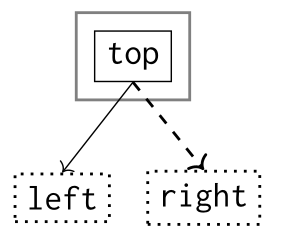
\includegraphics[width=0.2\linewidth]{Imagens/No-Normal} & 
        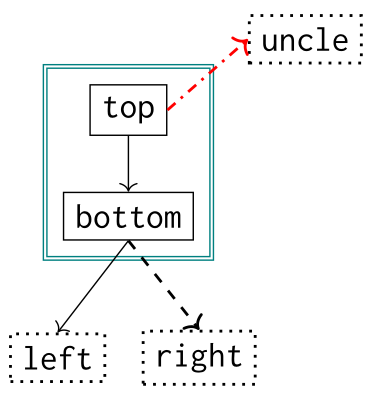
\includegraphics[width=0.2\linewidth]{Imagens/No-Skip} & 
        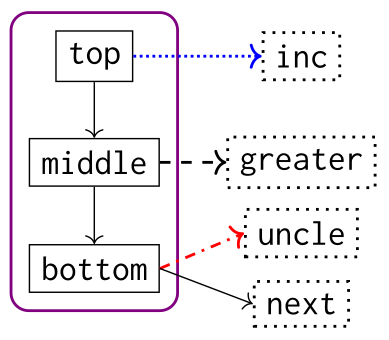
\includegraphics[width=0.2\linewidth]{Imagens/No-Leaf}\\
        Nós Normais & Nós \textit{Skip} & Nós Folha\\ 
    \end{tabular}
    \caption{Tipos de Nós}
    \label{tab:nos}
\end{figure}



\subsubsection{Construção}

Antes de discutir a construção é importante primeiro compreender os seguintes conceitos:
\begin{itemize}
    \item \textit{Right-Handed Depth} (RHD) -- Corresponde à distância do ancestral mais próximo que é um filho esquerdo.
    \item \textit{Right-Edge Depth} (RED) -- Corresponde à distância ao ancestral mais próximo que se encontra no caminho mais à direita a partir da raiz da árvore.
    \item \textit{Target uncle} -- Durante o algoritmo de \textit{lookup}, o \textit{target uncle} refere-se à criança direita do nó ancestral comum entre o nó de origem e o nó de destino.
\end{itemize}

A construção da Advanced Myers List perde a função de cons em tempo constante, pois exige saber previamente o número exato de elementos para calcular a altura da árvore lógica e formar uma árvore binária perfeita, utilizando elementos que servem como enchimento (\textit{fillers}) caso necessário.
A estrutura é construída recursivamente do \texttt{head} até a camada de folhas e a atribuição dos apontadores depende do tipo de nó:

\begin{itemize}
    \item Nós normais e \textit{skip}: O apontador \texttt{next} aponta para a sub-árvore esquerda e o \texttt{jump} para a sub-árvore direita
    \item Nós \textit{skip} e folhas: O apontador \texttt{uncle} liga a um tio onde a regra $\text{RED}(\texttt{s.uncle}) = \text{RHD}(\texttt{s})$ é verificada
    \item Nós folha: O apontador \texttt{inc} liga a uma folha mais próxima à direita tal que $\text{RHD}(f') = \text{RHD}(f) + 1$. O apontador \texttt{greater} liga à folha mais próxima à direita onde $\text{RHD}(f') > \text{RHD}(f)$, este apontador pode ser obtido recorrendo ao processo usado para o apontador \texttt{jump}.
\end{itemize}

\subsubsection{\textit{Lookup}}

O algoritmo de \textit{lookup} na Advanced Myers List determina dinamicamente o percurso ideal com base na posição relativa entre a célula de origem e a de destino, ramificando-se em três cenários fundamentais:

\begin{itemize}
    \item Descida Direta: Se o destino é um descendente direto da origem na árvore lógica, o algoritmo realiza uma descida através dos apontadores até alcançar o índice pretendido;
    \item Salto via \texttt{uncle}: Se existir um nó \textit{skip} ou folha descendente da origem cujo RHD coincida com o RED do \textit{target uncle}, o algoritmo salta diretamente para o \textit{target uncle} através do apontador \texttt{uncle};
    \item Travessia Lateral: Caso as condições de descendência não se apliquem, o algoritmo recorre aos apontadores \texttt{inc} para navegar horizontalmente entre nós folha adjacentes, ou ao apontador \texttt{greater} para saltar para a extremidade da subárvore corrente antes de transitar para a região seguinte da lista;
    \item Transição Ascendente: Quando nenhum dos três cenários anteriores é aplicável (por exemplo, quando a origem é uma folha cujo RHD já excede o RED necessário para o \textit{target uncle}), o algoritmo segue o apontador \texttt{next} para avançar para um nó não-folha. A partir dessa nova posição, é garantido que um dos três primeiros cenários será acionado.
\end{itemize}

\textbf{NOTA:} Aqui explicamos o funcionamento da Improved Myers List e da Advanced Myers List de uma forma muito superficial mas rápida de compreender, para uma compreensão e para um estudo mais informativo recomenda-se ler o artigo original.
